\chapter{Preliminares}\label{chapter:preliminaries}

El objetivo de este trabajo es diseñar e implementar un sistema que permita encontrar el sistema de ecuaciones diferenciales lineales con respecto a los parámetros que mejor ajuste un conjunto de datos. Para ello se propone usar algoritmos genéticos para resolver un problema de regresión simbólica. En este capítulo se presentan las ecuaciones diferenciales lineales con respecto a los parámetros, el ajuste mínimo cuadrático de datos, la regresión simbólica, los algoritmos genéticos y los splines de suavizado.

Los posibles sistemas se representan mediante árboles (que tienen una estructura dada, para garantizar que los sistemas siempre sean lineales en los parámetros) y sobre el espacio de estos árboles se aplica un algoritmo genético para determinar cuál de ellos es el que mejor ajusta los datos. Para determinar cuan cercano están los datos observados a los datos evaluados en uno de esos sistemas se resuelve un problema de ajuste mínimo cuadrático de datos, que al ser lineal los modelos, se reduce a la solución de un sistema de ecuaciones lineales. El método que se utiliza para la solución del problema mínimo cuadrático de datos asume que los datos son exactos (sin ruido). Cuando los datos observados tienen ruido el algoritmo obtiene sistemas con valores de ajustes que no interesan en el estudio. Para solucionar este valor en el ajuste lo que se hace es aproximar los datos con ruido con un spline de suavizado, y se aplica el método de ajuste mínimo cuadrático a los valores de los datos evaluados en el spline.

En la sección \ref{section:differential_equation_lineal_in_params} se presentan las ecuaciones diferenciales lineales con respecto a los parámetros. El ajuste mínimo cuadrático de datos, la regresión y la regresión simbólica se presentan en las secciones, \ref{section:min_square} y \ref{section:symbolic_regression}. En la sección \ref{section:symbolic_regression_in_does} se describe cómo se puede aplicar la regresión simbólica para encontrar el lado derecho de ecuaciones direrenciales. En la sección \ref{section:genetic_algorithm} se presentan los elementos fundamentales de los algoritmos genéticos. Finalmente en la sección \ref{section:smoothing_splines} se presentan los splines y los splines de suavizado.

\section{Ecuaciones diferenciales lineales con respecto a los parámetros}\label{section:differential_equation_lineal_in_params}

La modelación a través de ecuaciones diferenciales posibilita tanto la descripción como la predicción del desarrollo de fenómenos \cite{zill2012first}. La transferencia de calor \cite{p-transferencia-calor}, la transferencia de masa \cite{p-transferencia-masa}, el desarrollo de una población \cite{p-desarrollo-poblacion}, las relaciones amorosas \cite{p-amor}, el desarrollo de enfermedades como el VIH-SIDA \cite{p-desarrollo-vih}, el cólera \cite{p-desarrollo-colera}, la peste bubónica \cite{p-desarrollo-peste} o el COVID-19 \cite{p-desarrollo-covid} se estudian utilizando sistemas de ecuaciones diferenciales.

Una ecuación diferencial se define como una ecuación que contiene las derivadas de una o más variables dependientes, con respecto a una o más variables independientes \cite{gaucel2014learning}. Una ecuación diferencial ordinaria (EDO) es una que contiene derivadas de una función de una sola variable (por ejemplo, el tiempo). La forma general de una ecuación diferencial ordinaria es:

$$y'(t)=f(t, y(t)), \qquad y(t_0) = y_0$$

donde $y(t)$ es una función y $y_0$ es una condición inicial. A $f(t, y(t))$ se le llama parte derecha de la ecuación diferencial.

La solución de una ecuación diferencial es una función que al ser sustituida en la ecuación hace que se satisfaga dicha ecuación. Si además, la ecuación diferencial es ordinaria, su parte derecha es continua en un intervalo cerrado y se tienen condiciones iniciales, entonces la solución de dicha ecuación diferencial existe y es única \cite{zill2012first}. Un ejemplo de ecuación diferencial ordinaria es:

$$y' = x * y^{\frac{1}{2}}$$

en donde la solución sería

$$y = \frac{1}{16} * x^4.$$

Una ecuación diferencial puede tener parámetros, de ser así la función $f$ se escribe como $f(t, y(t), a)$ donde $a$ es un parámetro. Una ecuación diferencial es lineal con respecto a los parámetro si es de la forma

$$\frac{dX}{dt} = \sum_{i=1}^{n} a_i * f_i(t, y(t))$$

donde los $a_i$ son parámetros y todas las funciones $f_i(t,y)$ dependen de la variable $t$, de la variable $y$, pero no dependen de ningún parámetro $a_i$.

Esta definición se puede extender a sistemas de ecuaciones diferenciales si todas las ecuaciones cumplen esta propiedad.

Con ecuaciones diferenciales lineales en los parámetros se pueden modelar diversas situaciones como sistemas dinámicos poblacionales como el sistema de Lotka Volterra \cite{Hoppensteadt:2006}:

$$X' = \alpha * X - \beta * X * Y$$
$$Y' = \delta * X * Y - \gamma * Y$$

En ocasiones no es suficiente con saber que una EDO describe un fenómeno, porque los parámetros juegan un papel importante, como las tasas de infección \cite{weiss2013sir}, la interación entre especies \cite{gaucel2014learning} y la tasa de fallecidos por causas naturales \cite{kuddus2021mathematical}. En la práctica estos parámetros no tienen por qué conocerse a priori, y lo único que poseen los investigadores son observaciones en el tiempo del fenómeno que están estudiando. Sin embargo, a partir de estas observaciones del fenómeno, se pueden determinar los valores de los parámetros. una de las formas de hacer eso es mediante el ajuste mínimo cuadrático de datos.

\section{Ajuste mínimo cuadrático de datos}\label{section:min_square}

El método de ajuste mínimo cuadrático de datos es un caso particular de regresión. Una regresión es un conjunto de procesos estadísticos para estimar las relaciones entre una o más variables dependientes y una o más variables independientes. La relación que se busca se modela en forma de función paramétrica escogida de antemano por el investigador \cite{johnson2015applied}.

Dado un conjunto de $n$ muestras de $m$ variables independientes $x_i$ y el correspondiente valor de las $d$ variables dependientes $y_i$, $\{(x_i, y_i)\}^n_{i=1} \subset \mathbb{R}^m \times \mathbb{R}^d$, un vector de $k$ parámetros $\Theta \subset \mathbb{R}^k$ y una función $F : \mathbb{R}^{k + m} \rightarrow \mathbb{R}^d$ se define una función de ajuste como una función $E(y_i, f_i)$, donde $y_i$ es el valor de las variables dependientes observado con las variables independientes $x_i$, y $f_i = F(\Theta, x_i)$ es el valor estimado.

El problema de la regresión consiste en \textit{ajustar los datos}: encontrar los valores de los $k$ parámetros $\theta_1, \theta_2, \dots, \theta_k$ que minimicen la función de ajuste $E$
\begin{equation*}
    e = min_{\theta \in \Theta} \; E(y_i, f_i),
\end{equation*}

donde $e$ es el error de ajuste \cite{statisticintroductions}. Mientras más pequeño es el valor de $e$, mejor se considera el ajuste.

El método de ajuste mínimo cuadrático se utiliza para aproximar la solución de modelos en los que se conoce la forma general de la función que describe los datos observados, pero no los parámetros de esta función conocida.

Este método de ajuste se puede expresar como: resolver el problema de optimización de encontrar los valores de los $k$ parámetros $\theta_1, \theta_2, \dots, \theta_k$ que minimizan $S$ dado el modelo $f$ (que depende de los parámetros $\theta$) y los puntos $(xi, yi)$ donde:

$$S = \sum_{i=1}^{n}(y_i - f(x_i, \theta))^2.$$

Se define el valor de $S$ como error cuadrático medio.

Cuando se resuelve el problema de optimización, se obtiene el vector de parámetros $\theta$ y se puede estimar la variable dependiente cuando las variables independientes toman cualquier valor, incluso si no pertenecen al conjunto inicial. El ajuste mínimo cuadrático de datos se utiliza cuando se conoce la forma general de la función que describe los datos observados, pero hay ocasiones en la práctica en las que la función no se conoce, por ejemplo, el sistema de ecuaciones diferenciales que describe el virus COVID-19 no se ha encontrado, solo existen aproximaciones para modelar posibles escenarios de la enfermedad con el fin de ayudar en la creación de estrategias \cite{kuddus2021mathematical}. Para encontrar la función que describe los datos observados se puede utilizar la regresión simbólica.

\section{Regresión simbólica}\label{section:symbolic_regression}

La regresión simbólica consiste en encontrar una expresión matemática, en forma simbólica, que ajuste, de la mejor manera posible, un conjunto de observaciones. La introducción de la regresión simbólica generalmente se atribuye a John R. Koza \cite{zelinka2005analytic} quien mostró que puede usarse para descubrir modelos matemáticos mediante la codificacion de expresiones matemáticas como árboles computacionales.

En estos árboles, los nodos internos representan funciones ($+$, $-$, $*$, etc) que se extraen de un conjunto predeterminado de posibilidades, y los nodos hojas representan variables o constantes ($x_1$, $x_2$, $\dots$, $-1$, $\pi$, etc). Por ejemplo, la expresión:

$$a_1 y_1 + a_2 -(y_1 y_2),$$

se representa con el árbol computacional que aparece en la figura \ref{tikzpicture:koza_tree_example}.

\begin{center}
    % \begin{adjustbox}{width=0.35\textwidth, keepaspectratio}
    %     \begin{tikzpicture}[
    %             roundnode/.style={circle, draw, fill=gray!25, very thick, minimum size=7mm},
    %             squarednode/.style={rectangle, draw, fill=gray!25, very thick, minimum size=5mm},
    %         ]
    %         %Nodes
    %         \node[roundnode]      (plus)                             {$+$};
    %         \node[roundnode]           (star1)   [below left=of plus]    {$*$};
    %         \node[squarednode]         (a_1)   [below left=of star1]    {$a_1$};
    %         \node[squarednode]         (y_1)     [below=of star1]         {$y_1$};
    %         \node[roundnode]           (star2)   [below right=of plus]   {$*$};
    %         \node[squarednode]         (a_2)    [below left=of star2]    {$a_2$};
    %         \node[roundnode]           (neg)     [below=of star2]         {$-$};
    %         \node[roundnode]           (star3)   [below=of neg]         {$*$};
    %         \node[squarednode]         (y_1_2)   [below=of star3]   {$y_1$};
    %         \node[squarednode]         (y_2)     [below right=of star3]   {$y_2$};

    %         %Lines
    %         \draw[->] (plus.south) -- (star1.north);
    %         \draw[->] (plus.south) -- (star2.north);
    %         \draw[->] (star1.south) -- (a_1.north);
    %         \draw[->] (star1.south) -- (y_1.north);
    %         \draw[->] (star2.south) -- (a_2.north);
    %         \draw[->] (star2.south) -- (neg.north);
    %         \draw[->] (neg.south) -- (star3.north);
    %         \draw[->] (star3.south) -- (y_1_2.north);
    %         \draw[->] (star3.south) -- (y_2.north);
    %     \end{tikzpicture}%
    % \end{adjustbox}
    \begin{figure}[h]
        \centering
        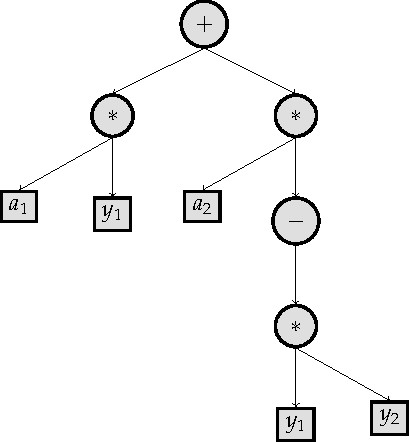
\includegraphics[width=0.4\textwidth]{"figures/koza_tree_example.pdf"}
        \caption{Ejemplo de árbol computacional que planteó Koza.}
        \label{tikzpicture:koza_tree_example}
    \end{figure}
\end{center}

En lugar de imponer una estructura de modelo que se considere matemáticamente manejable desde una perspectiva humana, en la regresión simbólica se consideran múltiples modelos evaluando su calidad con respecto a alguna métrica que es alguna variante del error cuadrático medio.

La definición matemática de la regresión simbólica es minimizar en $f$ la suma de $(f_i - y_i)^2 + penalization(f)$ donde $f$ es el conjunto de todos los árboles que representan los modelos de interes y $penalization$ es una función que penaliza alguna característica en los modelos, por ejemplo, la cantidad de nodos del árbol.


% Para evaluar que tan cercano está el modelo obtenido con respecto al modelo original se define una función de ajuste. La función de ajuste hace que los resultados obtenidos a lo largo de la regresión simbólica se acerquen más a la solución deseada ya que tiene en cuenta no solo las métricas de error (valores que definen cuán cerca están los resultados obtenidos a los resultados deseados), sino cualquier métrica que desee definir el usuario con el objetivo de obtener un resultado con características específicas, por ejemplo modelos más pequeños o con menor cantidad de parámetros. Esto facilita el análisis posterior de los resultados al permitir, en el modelo obtenido, asociar algunos parámetros a significados de la vida real, por ejemplo la cantidad de individuos que mueren en cada instante de tiempo en el sistema de lotka volterra.

La regresión simbólica tiene la desventaja de ser un problema NP-difícil \cite{virgolin2022symbolic} y contar con un espacio de búsqueda que abarca todas las funciones que van de $\mathbb{R}^m$ a $\mathbb{R}^n$. Sin embargo, poseer este espacio de búsqueda permite que el resultado puedan ser múltiples modelos y sus correspondientes conjuntos de parámetros. Examinar la colección de modelos resultantes permite al usuario identificar una solución que se ajuste mejor a algunas características en particular. Por ejemplo, que el modelo posea ecuaciones con poca cantidad de parámetros o que la diferencia entre los datos evaluados en el modelo y los datos originales sea menor que un error específico.

% tener un espacio de búsqueda mucho más grande que otros tipos de problemas de ajustes de datos. Por ejemplo, tanto en la regresión lineal como no lineal, el espacio de búsqueda es $\mathbb{R}^m$ y en la regresión simbólica se pueden explorar todas las funciones que van de $\mathbb{R}^m$ a $\mathbb{R}^n$.

% Sin embargo, la característica de poseer un espacio de búsqueda mayor a otros métodos también tiene ventajas, ya que el resultado pueden ser múltiples modelos y sus correspondientes conjuntos de parámetros. Examinar la colección de modelos resultantes permite al usuario identificar una solución que se ajuste mejor a algunas características en particular. Por ejemplo, que el modelo posea ecuaciones con poca cantidad de parámetros o que la diferencia entre los datos evaluados en el modelo y los datos originales sea menor que un error específico.

Se han desarrollado varios algoritmos para lidiar con el tamaño del espacio de búsqueda. Los enfoques fundamentales para la regresión simbólica son los algoritmos genéticos \cite{koza1994genetic, schmidt2013eureqa, gaucel2014learning}, recocido simulado \cite{turing_bot} y colonias de abejas \cite{multihive,karaboga2010artificial}. Dentro de los softwares utilizados para la regresión simbólica se encuentran \textit{gplearn} que es una biblioteca de código abierto desarrollada en el lenguaje de programación \textit{Python} \cite{gplearn}, \textit{Eureqa} es un sofware  comercial \cite{schmidt2013eureqa} y \textit{AI Feynman} es un método que utiliza un acercamiento mediante el uso de la técnica divide y vencerás \cite{udrescu2020ai}.

Existen trabajos en los que se ha usado la regresión simbólica para determinar el sistema de EDOs que mejor ajusta un conjunto de datos \cite{koza1994genetic, iba2008inference, gaucel2014learning, kronberger2019identification}. Para utilizar la regresión simbólica en EDOs se debe reducir el espacio de búsqueda a encontrar funciones desconocidas que representan el lado derecho de una ecuación diferencial. En la próxima sección se describe el problema de regresión simbólica para ecuaciones diferenciales ordinarias.

\section{Regresión simbólica para EDOs}\label{section:symbolic_regression_in_does}

Los sistemas de ecuaciones diferenciales permiten modelar fenómenos que ocurren en la sociedad y en la naturaleza \cite{weiss2013sir, udrescu2020ai, kuddus2021mathematical}. En ocasiones no se conoce con precisión el modelo de ecuaciones que está relacionado con los datos que describen al fenómeno, sería util disponer de un mecanismo para encontrar este modelo.

La regresión simbólica para EDO consiste en encontrar la parte derecha de una ecuación diferencial ordinaria, en forma simbólica, cuya solución sea una función que describa un conjunto de muestras. En este tipo de regresión simbólica, la función desconocida es el lado derecho de una ecuación diferencial. Se puede definir como que se tiene un conjunto de datos $N = \{(t_i, y_i)\}$ y se quiere encontrar la función $f(t, y(t))$ tal que la solución de:

\begin{equation*}
    \frac{dy}{dt} = f(t, y(t)),
\end{equation*}

sea una función $y$ tal que $y(t_i) \approx y_i, \forall(t_i, y_i) \in N$. Esta definición se puede extender a sistemas de EDOs.

La regresión simbólica permite encontrar una aproximación de una función $h$ dado un conjunto de datos de la forma $\{(t_i, h(t_i))\}$. Por lo que si se genera un conjunto de datos con la forma $S = \{((t_i, y(t_i)), f(t_i, y(t_i)))\}$ se puede utilizar la regresión simbólica para encontrar el valor de $f$.

La función $f$ está definida como la derivada de la función $y$, por lo que:

$$f(t_i, y(t_i)) = y'(t_i)$$

En \cite{gaucel2014learning, iba2008inference,kronberger2019identification} se aproxima el valor de la derivada de cada variable numéricamente por diferencias finitas. Con esta aproximación de la derivada se puede generar el conjunto $S$ y utilizar la regresión simbólica para encontrar una aproximación de $y$.

% En el año 1994 \cite{koza1994genetic}, John R. Koza definió que se podía utilizar la regresión simbólica para encontrar sistemas de ecuaciones diferenciales de forma automática.

En el año 2008 se utilizó la regresión simbólica junto con el algoritmo de mínimos cuadrados para encontrar el sistema de ecuaciones diferenciales lineales en los parámetros que mejor ajustase un conjunto de datos \cite{iba2008inference}. Una de las ventajas de estos sistemas es que, si los datos no presentan ruido, para encontrar sus parámetros solo es necesario resolver un sistema de ecuaciones lineales sobredeterminado \cite{myers2012generalized}.

% En el año 2014, un grupo de investigadores utilizaron la regresión simbólica para encontrar sistemas dinámicos. El acercamiento que utilizaron consistía en reducir el problema de regresión simbólica para sistemas de múltiples ecuaciones diferenciales en el problema de regresión simbólica para un sistema de una sola ecuación diferencial. De esta forma generaban para cada ecuación del sistema un grupo de ecuaciones y luego probaban distintas combinaciones de las ecuaciones de los subconjuntos obtenidos hasta encontrar la que mejor aproximase el conjunto de datos \cite{gaucel2014learning}.

% La investigación que se realizó en el año 2008 se utilizó en otro estudio correspondiente al año 2019. Los objetivos de ambas investigaciones son el mismo, en el estudio más reciente se sustituye el método de mínimos cuadrados para encontrar los parámetros por un algoritmo de descenso por gradientes \cite{kronberger2019identification}.

% Por un largo tiempo, la regresión simbólica solo era de dominio de los seres humanos, pero los estudios muestran cómo en las últimas décadas también se ha convertido en el dominio de los ordenadores. En la actualidad existen dos métodos que se utilizan en la regresión simbólica por medio de ordenadores. El primero se llama evolución gramatical y el segundo algoritmos genéticos \cite{zelinka2005analytic}. El último método se explicará en la siguiente sección.

En \cite{koza1994genetic, iba2008inference, gaucel2014learning, kronberger2019identification} se utilizan algoritmos genéticos para resolver el problema de la regresión simbólica. Esta solución a la regresión simbólica es la misma utlizada en este trabajo por lo que es necesario definir qué es un algoritmo genético. En la siguiente sección se define este tipo de metaheurística.

\section{Algoritmos genéticos}\label{section:genetic_algorithm}

Un algoritmo genético es una metaheurística inspirada en el proceso de selección natural \cite{mitchell1998introduction}. Este tipo de algoritmo genera posibles soluciones para el problema, a partir de las cuales se obtienen nuevas soluciones usando dos operacions: mutación y cruzamiento. en el cruzamiento se combinan dos soluciones para obtener una nueva, y en la mutación se obtiene una solución modificando otra. Este proceso (de cruzar y mutar) se repite hasta que se cumpla algún criterio de parada. En qué consisten las operaciones de cruzamiento y mutación dependen de cada problema específico.

El algoritmo genético es un proceso iterativo, en el que se toma una población inicial de individuos y se le aplican modificaciones generando nuevos individuos. De la población resultante se seleccionan algunos sujetos que pasarán a ser la población inicial de la siguiente iteración del método. La población de la primera iteración se genera creando individuos aleatoriamente. A cada iteración del algoritmo se le llama generación.

Los algoritmos genéticos se usan para resolver problemas de optimización de la forma $min f(x)$, donde $x$ pertenece a un conjunto $C$ dado. Se le llama solución a cualquier $x$ de $C$. En dependencia de la estructura de $C$, las soluciones pueden tener distintas formas, por ejemplo vectores de números reales como en los problemas de optimización de dimensión finita \cite{mitchell1998introduction} o pueden ser árboles como en el caso de la regresión simbólica \cite{mitchell1998introduction}.

El proceso de creación de nuevas generaciones se repite hasta que se alcanza una condición de parada. Algunas condiciones de parada comunes son \cite{mitchell1998introduction}:

\begin{itemize}
    \item Se encuentra un individuo lo suficientemente cercano a la solución del problema.
    \item Se alcanza el número máximo fijado de generaciones.
    \item Se alcanza la cantidad de tiempo o cómputo máximo asignado
    \item La cercanía de los individuos respecto a la solución del problema está alcanzando o ha alcanzado un nivel tal que las iteraciones sucesivas ya no producen mejores resultados.
    \item Combinaciones de las anteriores.
\end{itemize}

Para el proceso de modificación de la población de una generación se utilizan dos operadores: la mutación y el cruzamiento. Las operaciones se realizan sobre individuos aleatorios seleccionados de la población. La mutación realiza cambios aleatorios en alguna característica de un individuo seleccionado, y el cruzamiento intercambia características aleatorias de dos individuos seleccionados, obteniendo dos nuevos individuos. Existen operaciones de cruzamiento en la que solo se obtiene un nuevo individuo como resultado de la operación, este tipo de cruzaminento se utiliza en la propuesta de solución planteada en este trabajo.

Una realizado el proceso de modificación de la población mediante el uso de las operaciones de mutación y cruzamiento, se realiza la operación de selección. La operación escoge de la población inicial de la generación y del conjunto de individuos resultantes de las mutaciones y cruzamientos aquellos que se acerquen más a la solución del problema y un subconjunto de individuos aleatorios. La selección de individuos aleatorios se realiza con el fin de no caer en mínimos locales en la búsqueda de la solución que más se acerque a la solución del problema \cite{mitchell1998introduction}. En total, el proceso de selección escoge una cantidad de individuos igual a la población inicial de la generación \cite{mitchell1998introduction}.

Las operaciones de cruzamiento, mutación y selección dan como resultado la población de soluciones de la próxima generación. Dado que los individuos más cercanos a la solución del problema fueron escogidos en la operación de selección, la distancia del mejor individuo de la población a la solución nunca empeora entre cada generación.

% Con el fin de explorar de maneras distintas el espacio de búsqueda, vale la pena ajustar parámetros del algoritmo genético como la probabilidad de mutación, de cruzamiento y el tamaño de la población, para encontrar configuraciones adecuadas para la clase de problema en la que se trabaja. Los parámetros típicamente interactúan entre sí de forma no lineal, por lo que no se puede optimizar uno a la vez. Hay mucha discusión y enfoques para la selección de parámetros de los algoritmos genéticos en la literatura de computación evolutiva, pero no hay resultados concluyentes sobre lo que es mejor; la mayoría de los investigadores usan lo que funcionó bien en casos previamente informados \cite{mitchell1998introduction}.

Para evaluar que tan cercano se encuentra un individuo de la población a la solución se utiliza un función de ajuste, esta función de ajuste en el caso de estar resolviendo un método de regresión simbólica es mediante el ajuste mínimo cuadrático de datos. Como el espacio de búsqueda son los sistemas de ecuaciones diferenciales lineales en los parámetros, se pueden encontrar los parámetros presentes en el individuo mediante la solución de un sistema de ecuaciones lineales sobredeterminados si los datos no presentan ruido.

Si un conjunto de datos $\{x_i, Y_i\}$ que describen el fenómeno $f$ es de la forma $Y_i = f(x_i) + \epsilon _i$ donde los $\epsilon _i$ son valores aleatorios, independientes y con media 0, entonces se dice que el conjunto de datos posee ruido. Los datos que se utilizan para encontrar una solución en el algoritmo genético pueden poseer ruido. Altos niveles de ruido pueden ocasionar que el modelo seleccionado como solución no ajuste de forma correcta otros datos que describan el mismo fenómeno pero que no posean ruido. Para eliminar el término $\epsilon _i$ en los datos (eliminar el ruido en los datos) se pueden utilizan varias técnicas, una de estas técnicas son los Splines de suavizado.

\section{Spline de suavizado}\label{section:smoothing_splines}

Un spline es una función definida por intervalos, donde la función de cada intervalo es un polinomio. El máximo grado de los polinomios que se utilizan define el grado del spline \cite{ahlberg1967theory}. Los extremos de los intervalos se llaman ``nudos'' y el spline pasa por cada uno de los nudos seleccionados. La forma general de un spline cúbico es la expresión paramétrica:

$$S(t) = a_ix^3 + b_ix^2 + c_ix + d_i, \qquad t_i \leq t < t_{i+1}$$

Un spline de suavizado es un spline en el que los nudos son todos los puntos dados pero la curva resultante no pasa necesariamente por los nudos. El spline de suavizado cúbico $\hat{f}$ que aproxima el fenómeno $f$ se define como el resultado del problema de encontrar los parámetros $a_i, b_i, c_i, d_i$ que minimizan:

$$min \sum_{i=1}^n (Y_i - \hat{f}(x_i))^2 + \lambda \int \hat{f}''(x)^2 dx,$$

donde $\{(x_i, Y_i)\}$ es un conjunto de puntos con ruido que describe a $f$, y $\lambda$ se define como factor de suavizado y es mayor igual que 0. Si el factor de suavizado es 0, entonces el spline de suavizado coincide con el el spline donde se escogen como nudos todos los datos. A medida que el valor de $\lambda$ aumenta, el resultado se acerca a la aproximación de los datos por el método de mínimos cuadrados \cite{green1993nonparametric}. En la figura \ref{fig:spline_0.1} se puede ver un spline de suavizado con $\lambda=0.9$ y en la figura \ref{fig:spline_1} se puede ver un spline de suavizado con $\lambda=0$

\begin{figure}[h]
    \centering
    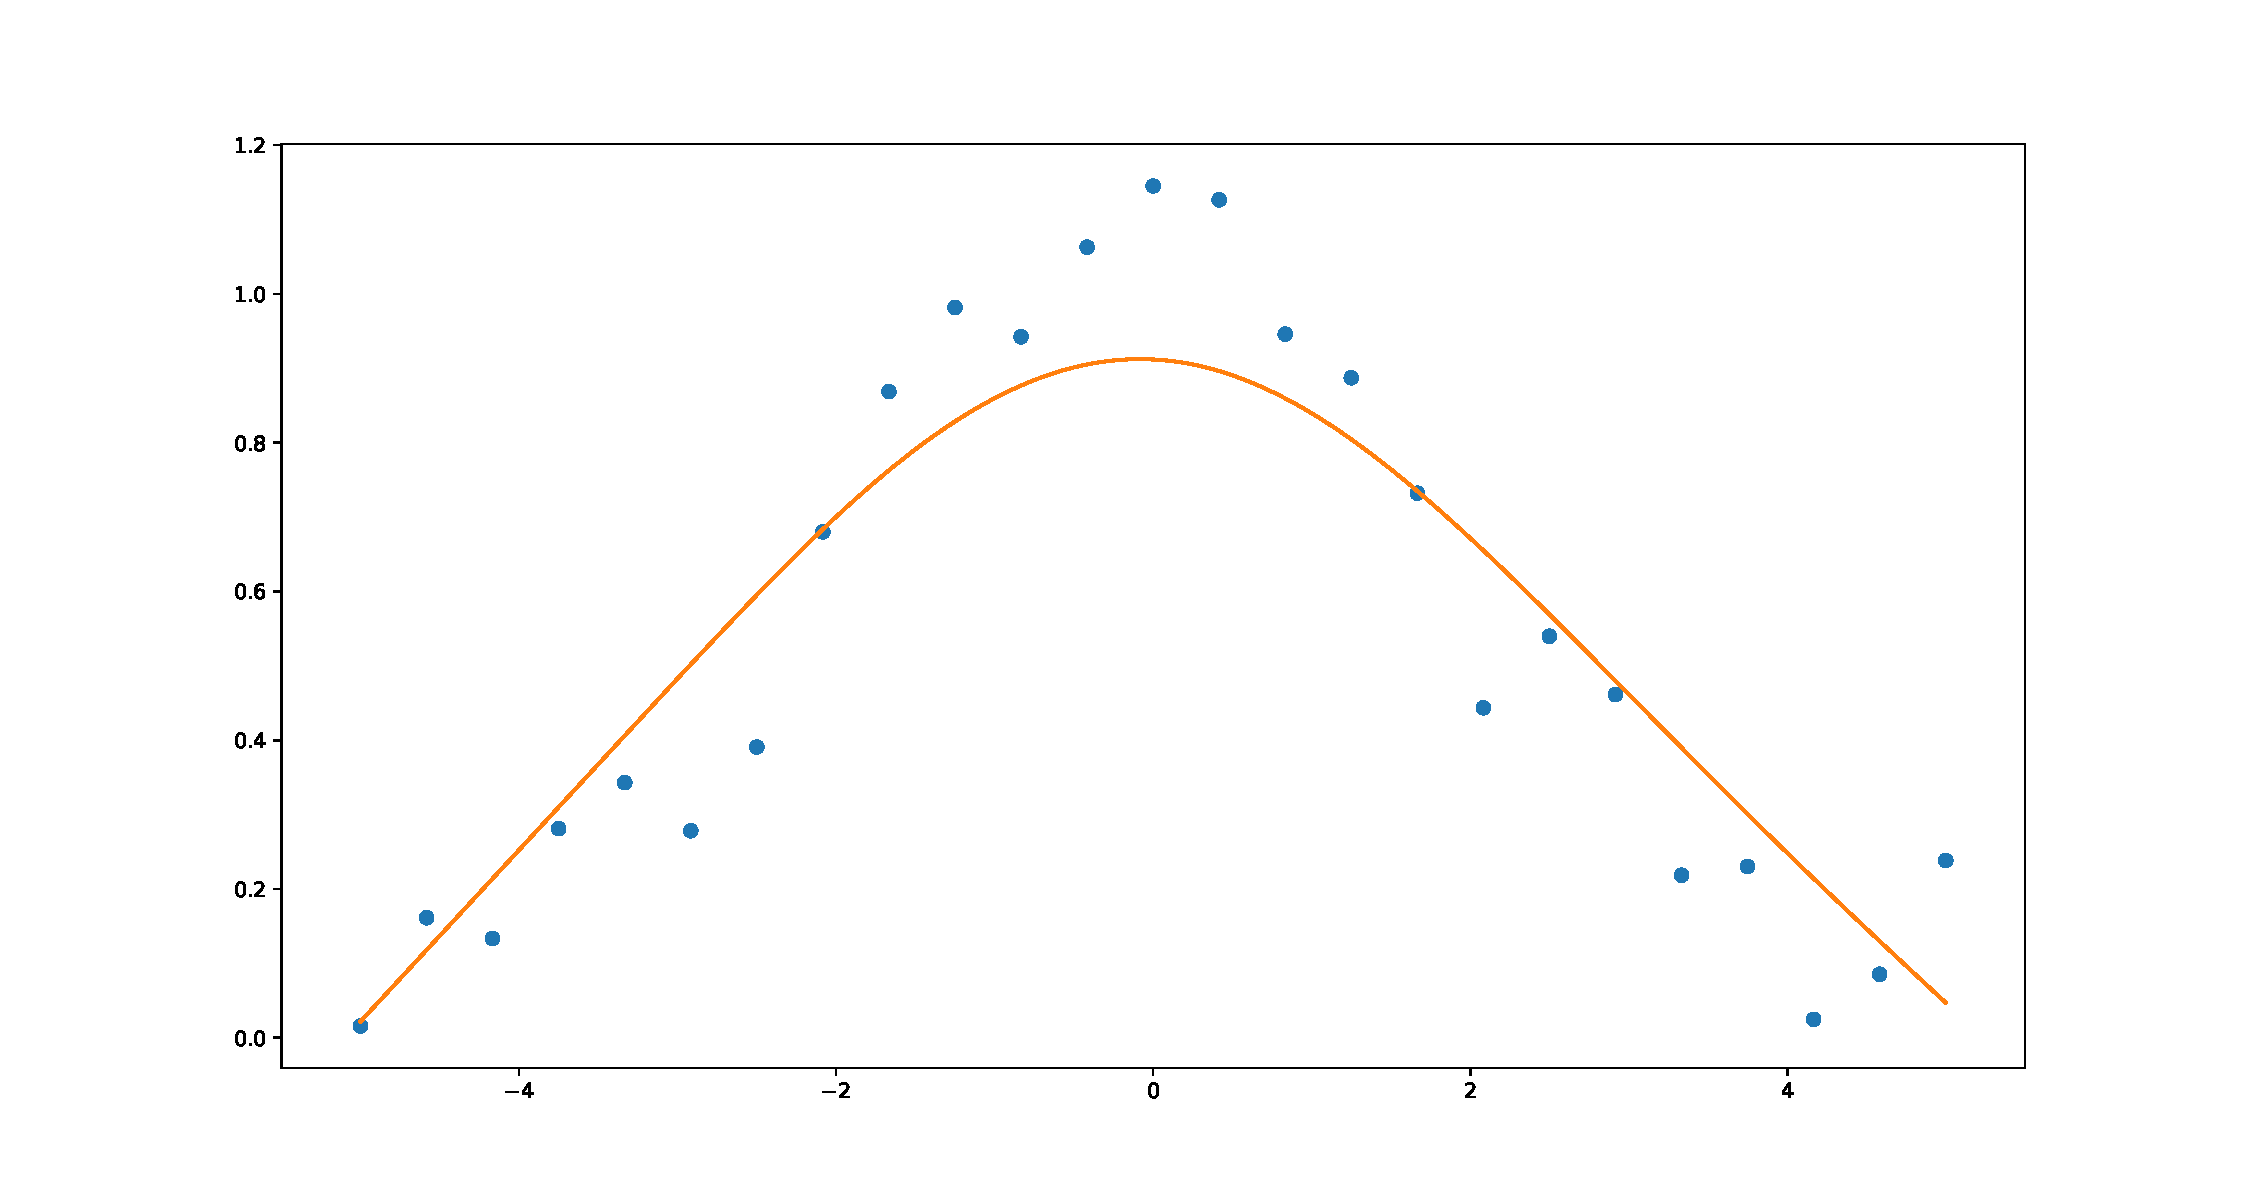
\includegraphics[width=\textwidth]{"figures/spline_0.1.pdf"}
    \caption{Spline de suavizado con $\lambda = 0.9$.}
    \label{fig:spline_0.1}
\end{figure}

\begin{figure}[h]
    \centering
    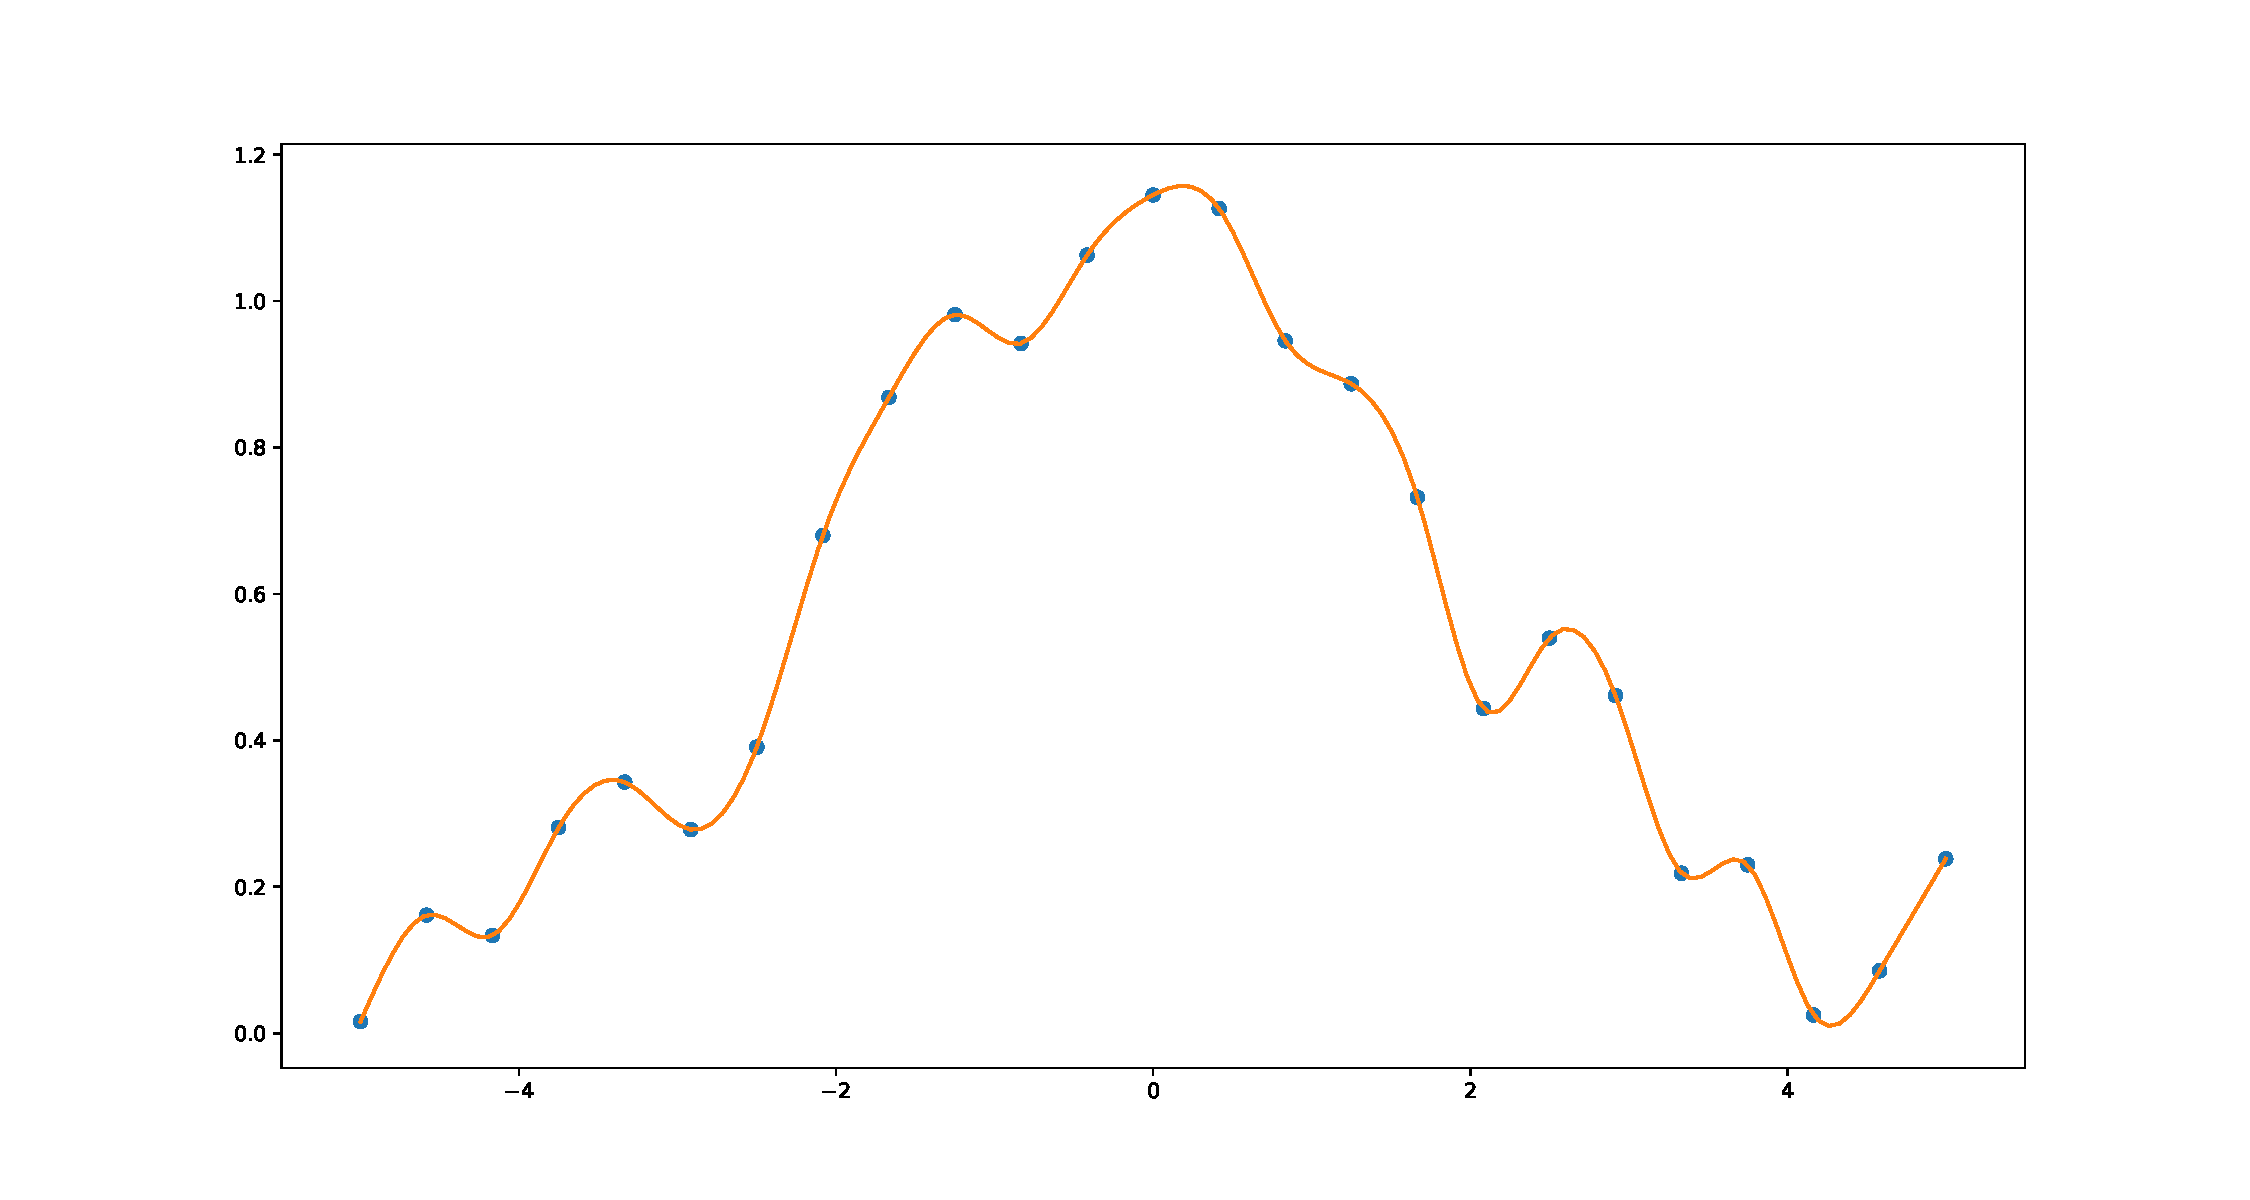
\includegraphics[width=\textwidth]{"figures/spline_1.pdf"}
    \caption{Spline de suavizado con $\lambda = 0$.}
    \label{fig:spline_1}
\end{figure}


Si se tiene un conjunto de puntos $\{(x_i, Y(x_i))\}$ con ruido, se puede utilizar un spline de suavizado cúbico para aproximar la función $Y$. Con este spline de suavizado se puede obtener una aproximación de $Y'$ y con esta derivada se puede emplear la regresión simbólica para encontrar el sistema de ecuaciones diferenciales lineales en los parámetros que ajuste el conjunto de datos.

En este capítulo se definieron conceptos utilizados en la propuesta de solución. La solución que se propone utiliza un spline de suavizado para la obtención de una aproximación de las derivadas de un conjunto de datos dado. Con las aproximaciones de las derivadas, se utiliza la regresión simbólica mediante un algoritmo genético para la obtención de un sistema de ecuaciones diferenciales lineales con respecto a los parámetros que ajuste el conjunto de datos. Para usar un algoritmo genético es necesario definir varios elementos:

\begin{itemize}
    \item Cuáles son las posibles soluciones
    \item Cómo aplicar un operador de cruzamiento
    \item Cómo aplicar un operador de mutación
    \item Cómo determinar cuán buena es una solución
    \item Cómo determinar qué soluciones pasan a las próximas generaciones
\end{itemize}

En el próximo capítulo se describe cómo se aplican estos elementos a la regresión simbólica para identificar sistemas de EDOs lineales con respecto a los parámetros.
